\documentclass[10pt]{beamer}

\usetheme{metropolis}
\usepackage{appendixnumberbeamer}

\usepackage{booktabs}
\usepackage[scale=2]{ccicons}
\usepackage{graphicx}
\usepackage{pgfplots}
\usepgfplotslibrary{dateplot}
\usepackage{caption}
\usepackage{subcaption}
\usepackage{xspace}
\usepackage{hyperref,xcolor}
\usepackage{textpos}

\usepackage{makeidx}
\definecolor{winered}{rgb}{0.5,0,0}
\newcommand{\themename}{\textbf{\textsc{metropolis}}\xspace}

\title{Bhabha Tracking Efficiencies}
%\subtitle{A modern beamer theme}
\date{12.04.2019}
\author{Martin Sobotzik}
\institute{Johannes Gutenberg Universit\"at Mainz}
% \titlegraphic{\hfill
\includegraphics[height=1.5cm]{logo.pdf}}

\definecolor{darkblue}{rgb}{0,0,.5}
\hypersetup{pdftex=true, colorlinks=true, breaklinks=true, linkcolor=darkblue, menucolor=darkblue, pagecolor=darkblue, urlcolor=darkblue}


%citecolor={winered} %Gives errors when turned on
%allcolors={winered} %Gives errors when turned on

\begin{document}

\maketitle
{%
\setbeamertemplate{frame footer}{Bhabha Tracking Efficiencies}

%\section{Reproducing Plots}


\begin{frame}{Motivation}

\begin{itemize}	
	\item I would like to estimate the tracking efficiency on phase 2 data
	\item I use Bhabha events because if one track is reconstructed then the other particle should also produce a track

\end{itemize}
	\begin{equation*}
		\epsilon = \frac{\textrm{Number of Bhabha events with exactly 2 tracks}}{\textrm{Number of Bhabha events with 1 or more tracks}}
	\end{equation*}
	
	\begin{itemize}
		\item  This idea comes from some plots presented by Sam Cunliffe in previous  \href{https://confluence.desy.de/display/BI/ECL+Meetings?preview=/84320165/109161400/SCunliffe181123-ECL.pdf}{tracking and ECL} meetings.
	\end{itemize}





\end{frame}
	
\begin{frame}{Getting Started}
	
\begin{itemize} 
	\item Cuts Sam used:
	
	
	\begin{itemize}
		\item $\textrm{gamma:probe}$ '$(\textrm{E} > 0.1 )$'
		\item $\textrm{gamma:tag}$ '$(\textrm{clusterE} > 3.0)$'
		\item $\textrm{vpho:cand}$ 'reconstructed from $\textrm{gamma:probe}$ and $\textrm{gamma:tag}$'
	\end{itemize}

	
		\begin{itemize}
			\item $0.296706 < \theta < 2.61799 \rightarrow$ It has to hit the ECL
			\item $\textrm{nCleanedTracks}[ \textrm{abs}(\textrm{dz}) < 2.0 \textrm{ and } \textrm{abs}(\textrm{dr}) < 0.5 \textrm{ and nCDCHits} > 0 \textrm{ and pt } > 0.15] < 1 \rightarrow $ bad quality hits 
						
		\end{itemize}
	
\end{itemize}

\begin{itemize}
	\item Cuts I use:
	\begin{itemize}
		\item $\textrm{M(vpho)}>8.0\, \textrm{GeV}$ $\rightarrow$ For the vpho to have a mass of at least $8\,\textrm{GeV}$, $\textrm{gamma:tag}$ and $\textrm{gamma:probe}$ must have at least an energy of more than $3\,\textrm{GeV}$
	
	\end{itemize}
\end{itemize}

	
\end{frame}

\begin{frame}{Reproducing Plots}
	
\begin{itemize}
	\item For data I using prod6 (this is because as a starting point I tried to reproduce Sam's plots)
	\item I am using the following data: /hsm/belle2/bdata/Data/release-02-01-00/DB00000438 /prod00000006/e0003/4S/r02*/all/mdst.sub00/*.root
\end{itemize}

	
	\begin{figure}
		\begin{subfigure}{.5\textwidth}
			\centering
			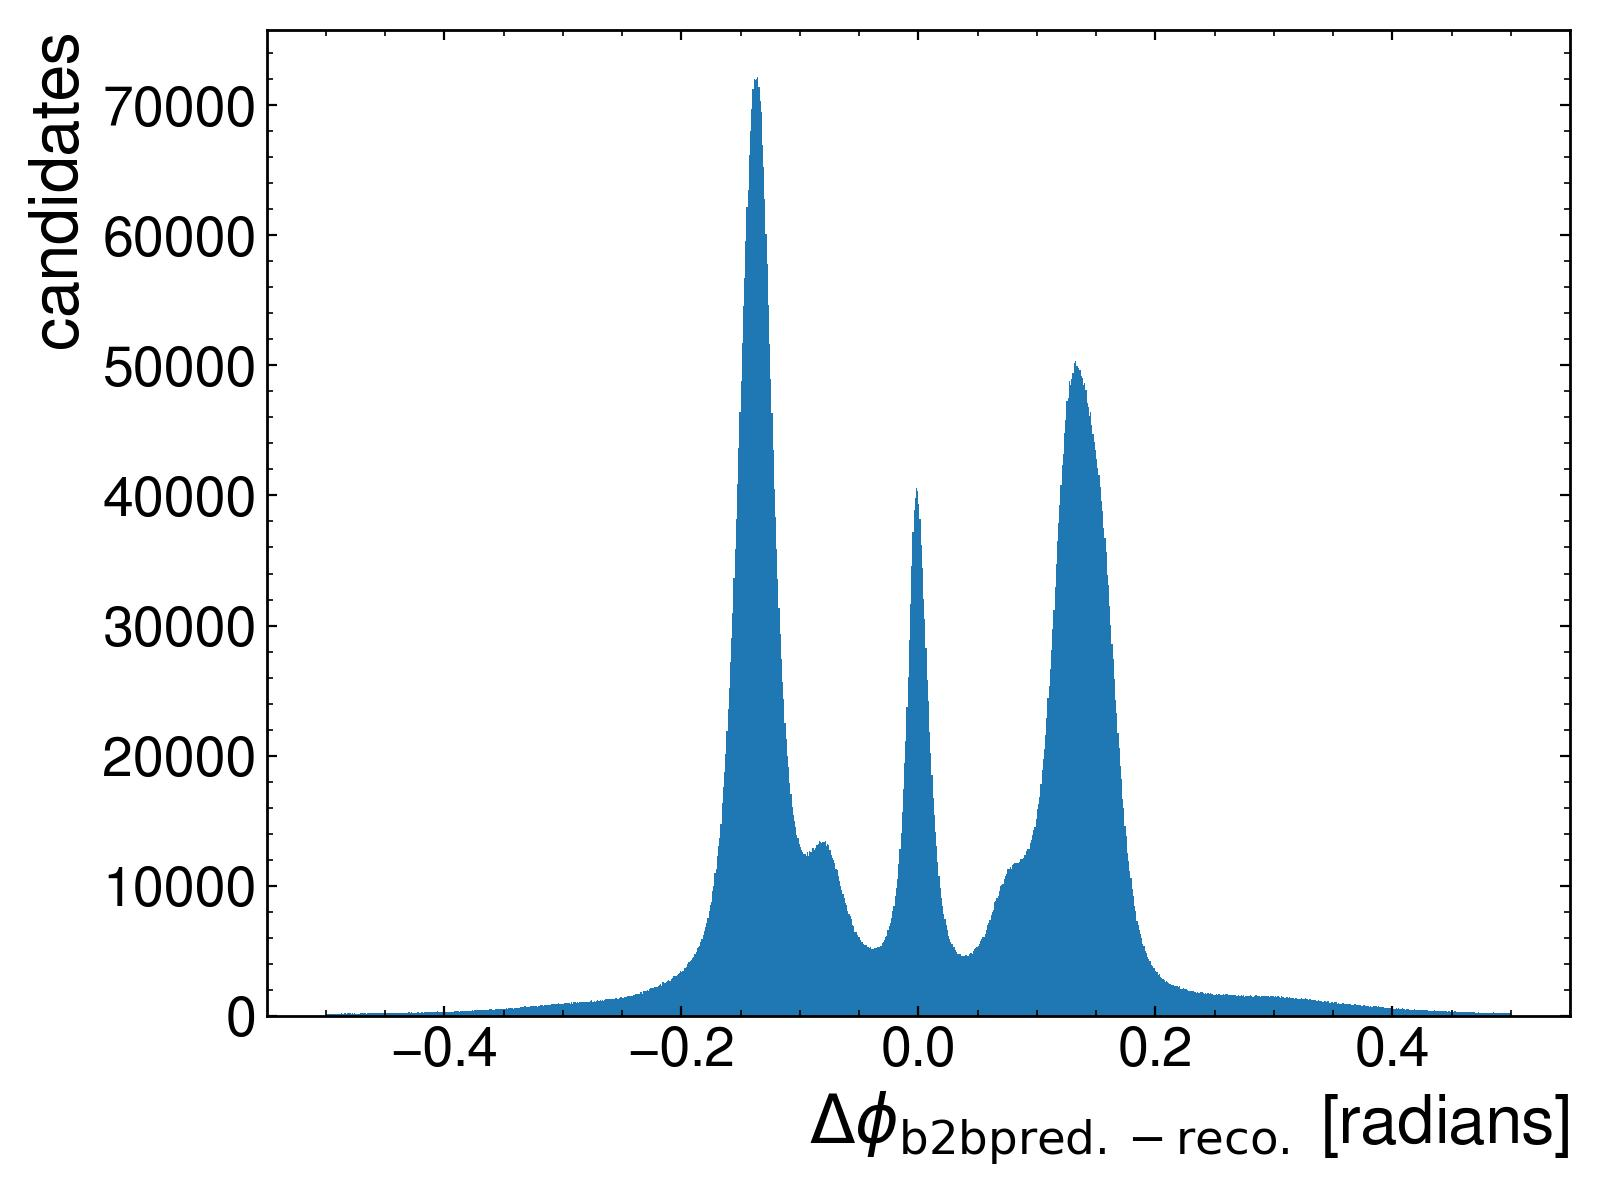
\includegraphics[width=4.5cm]{Plots/deltaPhiSam.jpeg}
			
			\label{fig:sub1}
		\end{subfigure}%
		\begin{subfigure}{.5\textwidth}
			\centering
			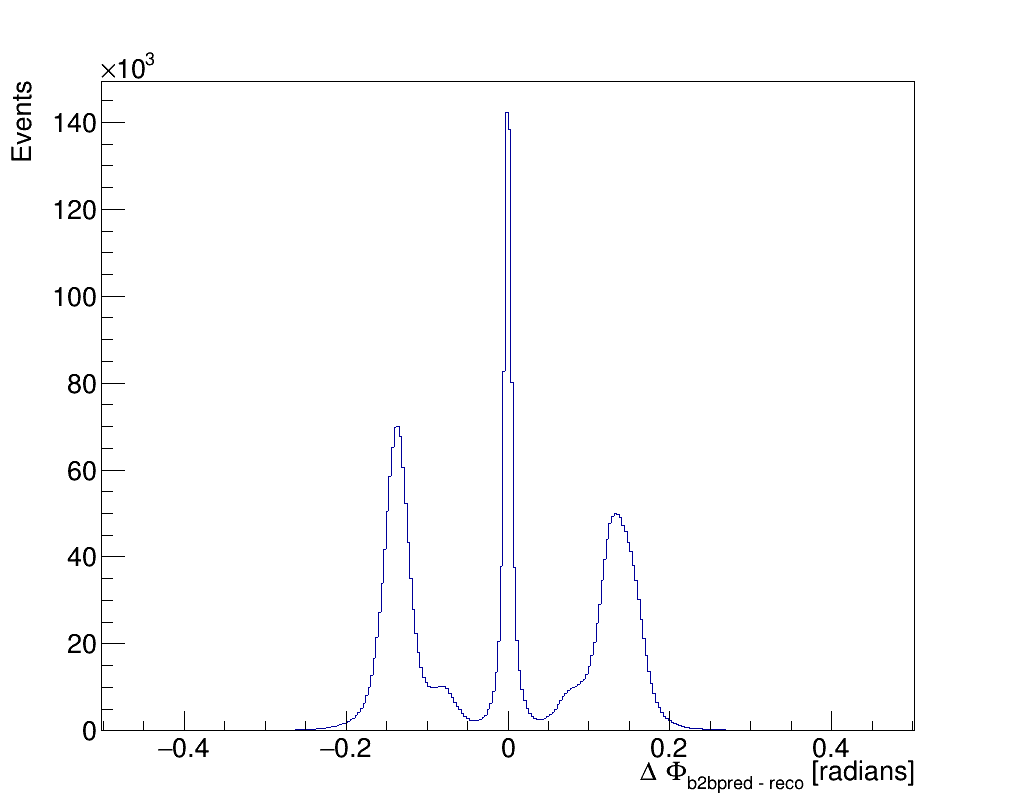
\includegraphics[width=4.5cm]{Plots/DeltaPhi.png}
			
			\label{fig:sub2}
		\end{subfigure}
		
		\label{fig:test}
	\end{figure}
	
	\begin{textblock*}{\textwidth}(1.7cm,-4.3cm)
		\textcolor{blue}{Sam: All data files}
	\end{textblock*}

	\begin{textblock*}{\textwidth}(7.8cm,-4.3cm)
		My
	\end{textblock*}
	
	
	
\end{frame}




\begin{frame}{Original idea}
		\begin{itemize}
			
		\item Treat every hit in the ECL as a photon
		\item After reconstruction, check if there is a track associated with the cluster
		
	\end{itemize}
	
\begin{figure}
	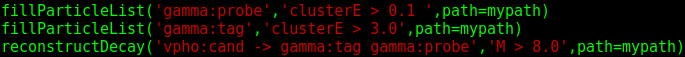
\includegraphics[width=11cm]{Plots/oldSc}
\end{figure}
\begin{itemize}
	\item As a first check I ran over MC11 $\textrm{ee}\rightarrow\textrm{ee}$ samples with the same steering file
	\item Far too few vpho were reconstructed and the daughters had no tracks associated
	\item Explanation: The $\gamma$ list is only filled by particles without a track
	\item So the reconstruction from two $\gamma$ lists is exactly what we don't need
\end{itemize}
\end{frame}



\begin{frame}{How to proceed}
	\begin{itemize}
		\item If there is a cluster in the ECL, we check if that cluster has a track associated. If it has than it is an $\textrm{e}^+/\textrm{e}^-$. If it has not then it is a $\gamma$ 
		\item So the list we want is a list filled with every event in the ECL 
		
		 
	\end{itemize}

\begin{figure}
	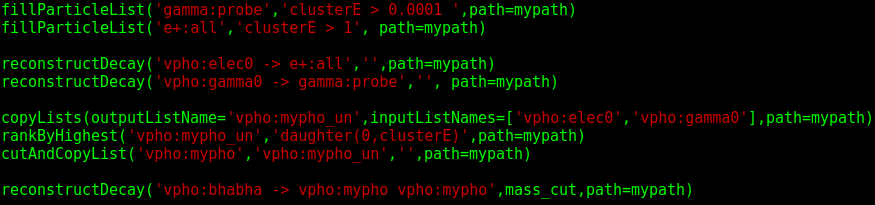
\includegraphics[width=11cm]{Plots/newSc}
\end{figure}

\begin{itemize}
	\item To add these two lists a \textit{pseudo} vpho has to be introduced 
	\item The vpho we want can then be reconstructed
\end{itemize}




\end{frame}

\begin{frame}{Running on MC}
	\begin{itemize}
		\item Running on MC11 $\textrm{ee}\rightarrow \textrm{ee}$ with new steering file
	\end{itemize}
	\begin{figure}
		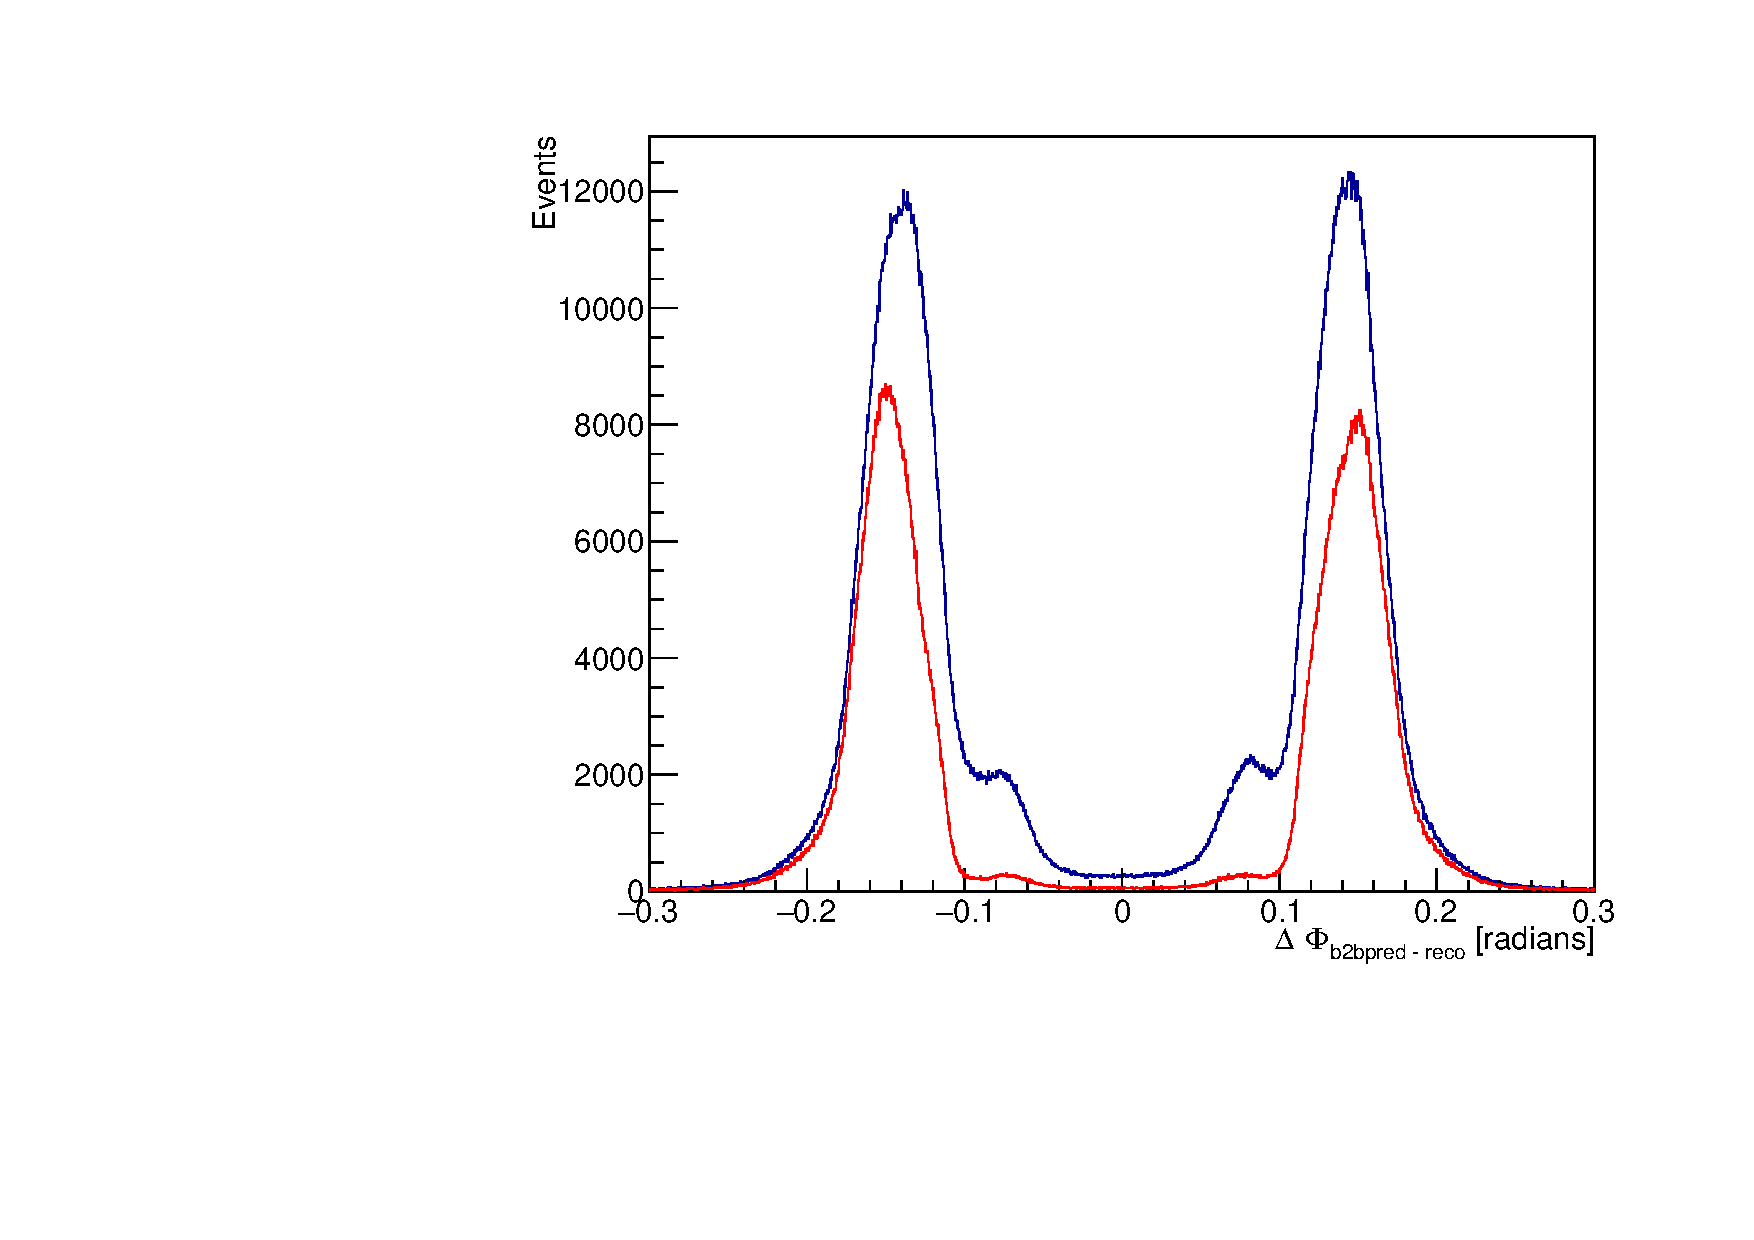
\includegraphics[width=5.5cm]{Plots/isSignalDeltaPhi}
	\end{figure}
\begin{itemize}
	\item Pure Bhabha sample $\rightarrow$ No middle peak caused by $\gamma \gamma$ events
	\item Difference between \textcolor{blue}{reconstructed} and \textcolor{red}{MCTruthMatched}  is caused by inefficiency
\end{itemize}

\end{frame}

\begin{frame}{Running on MC}
	
	\begin{textblock*}{\textwidth}(0cm,-3.8cm)
		\begin{figure}
			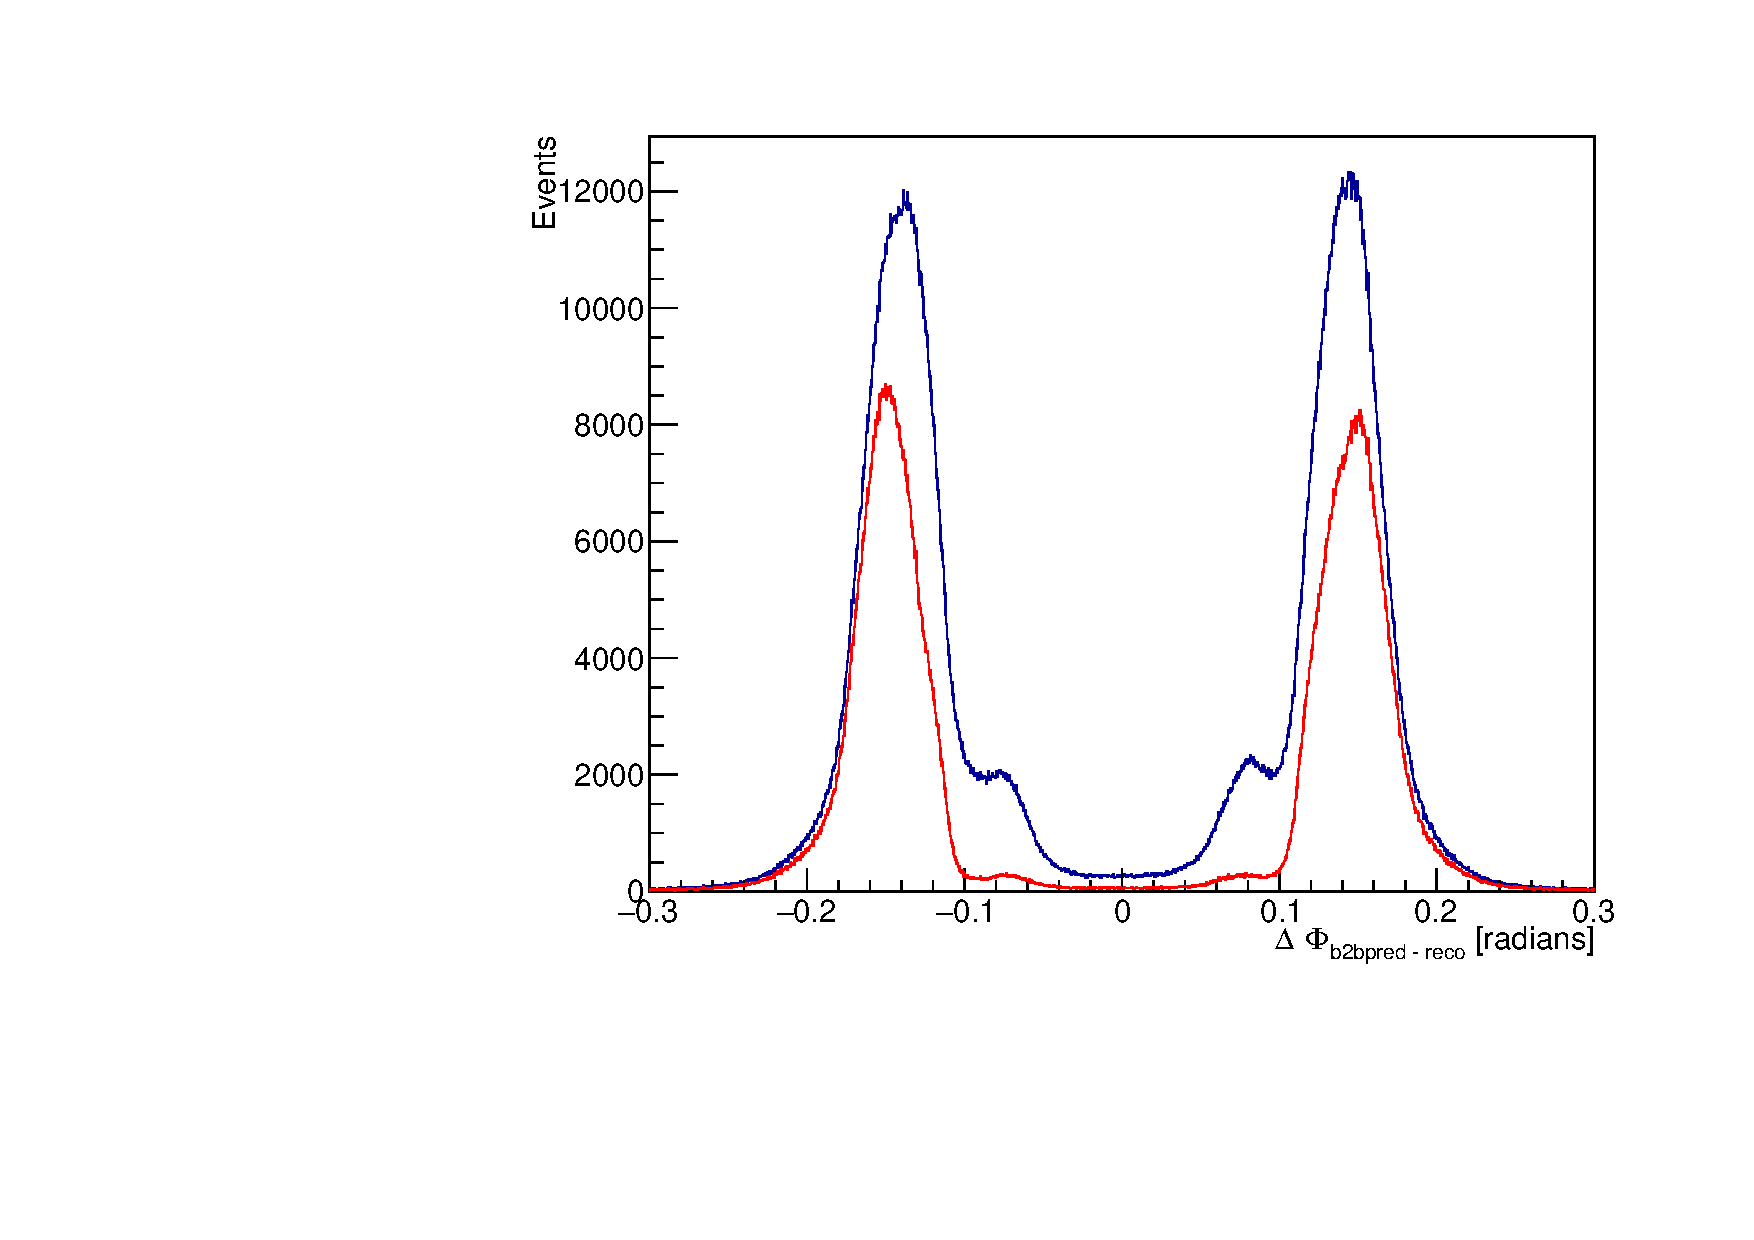
\includegraphics[width=4cm]{Plots/isSignalDeltaPhi}
		
		\end{figure}
	\end{textblock*}

\begin{textblock*}{\textwidth}(-4cm,-0.5cm)
	\begin{figure}
		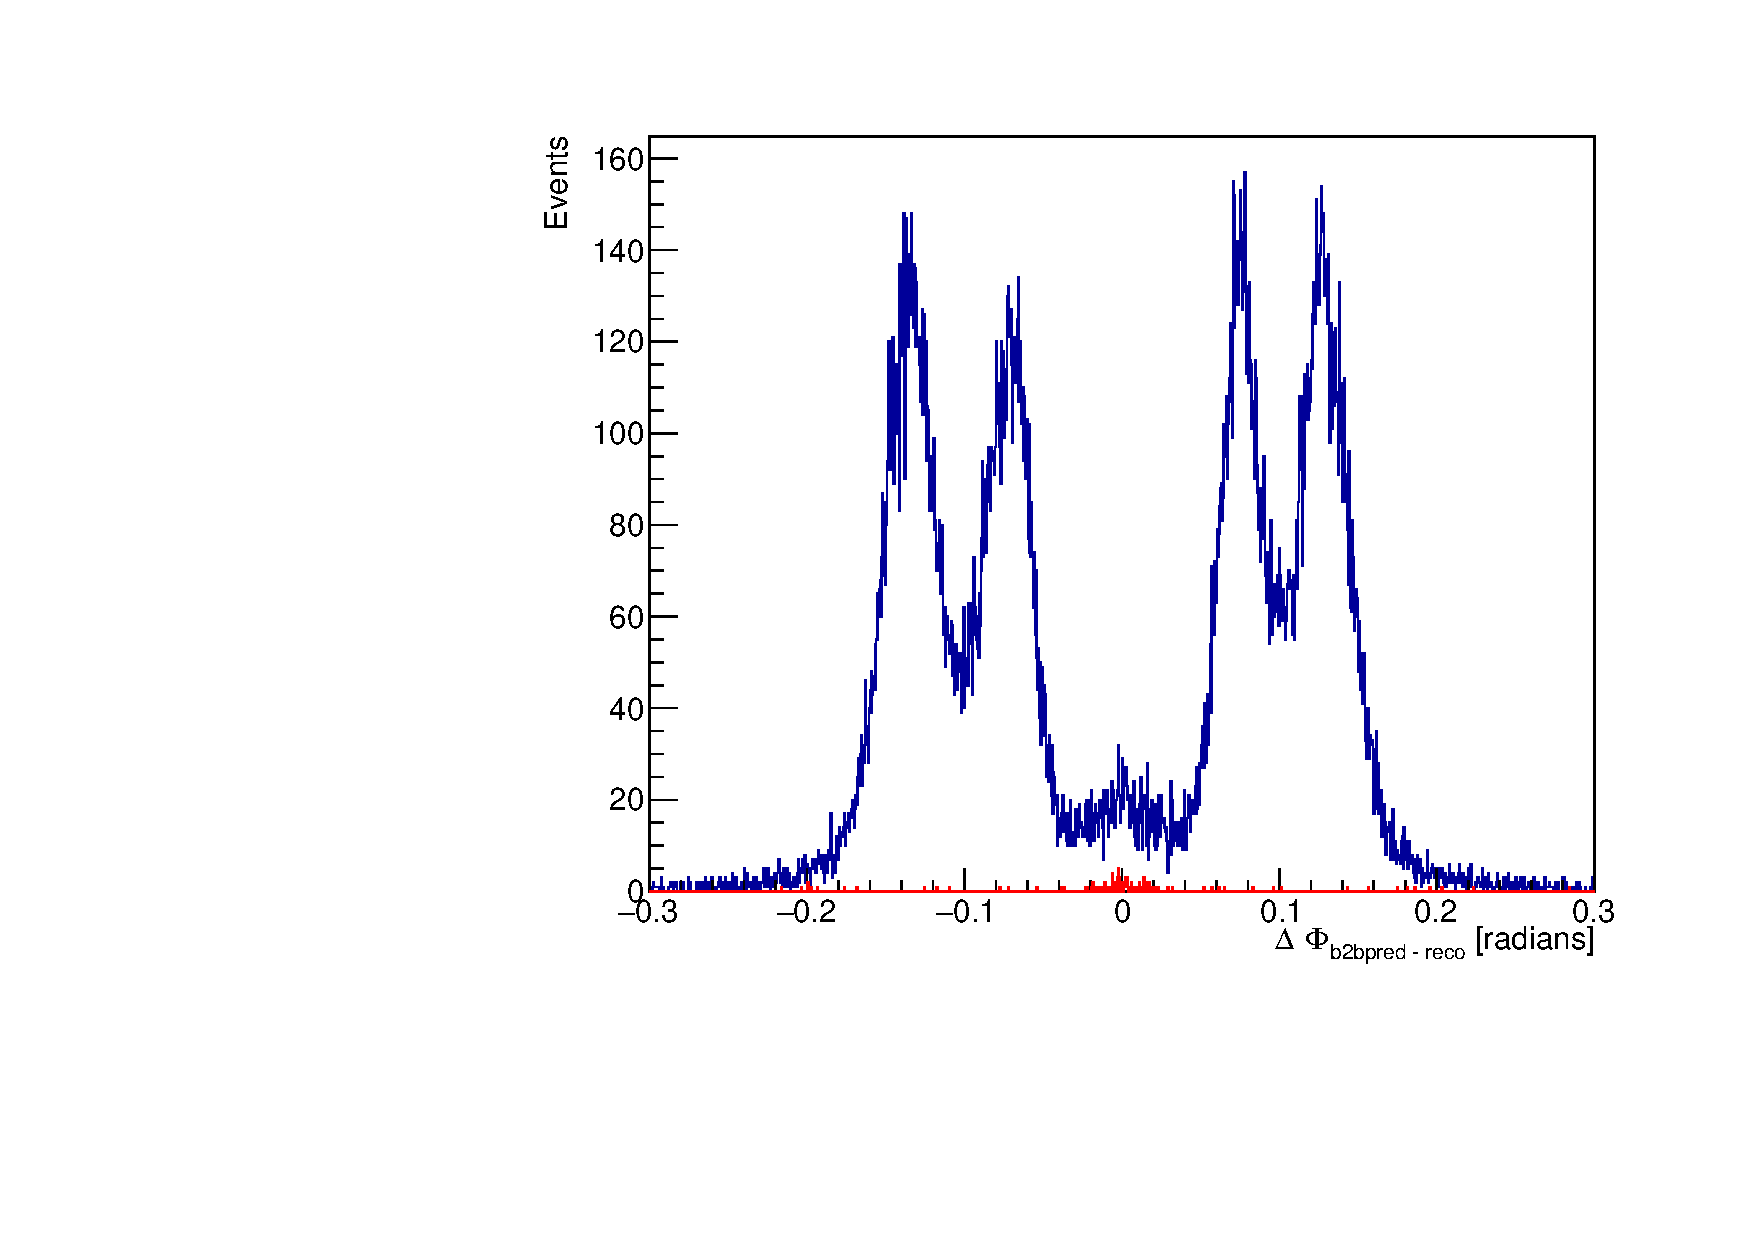
\includegraphics[width=4cm]{Plots/MCgg}
	\end{figure}
	
\end{textblock*}


\begin{textblock*}{\textwidth}(0cm,-0.5cm)
	\begin{figure}
		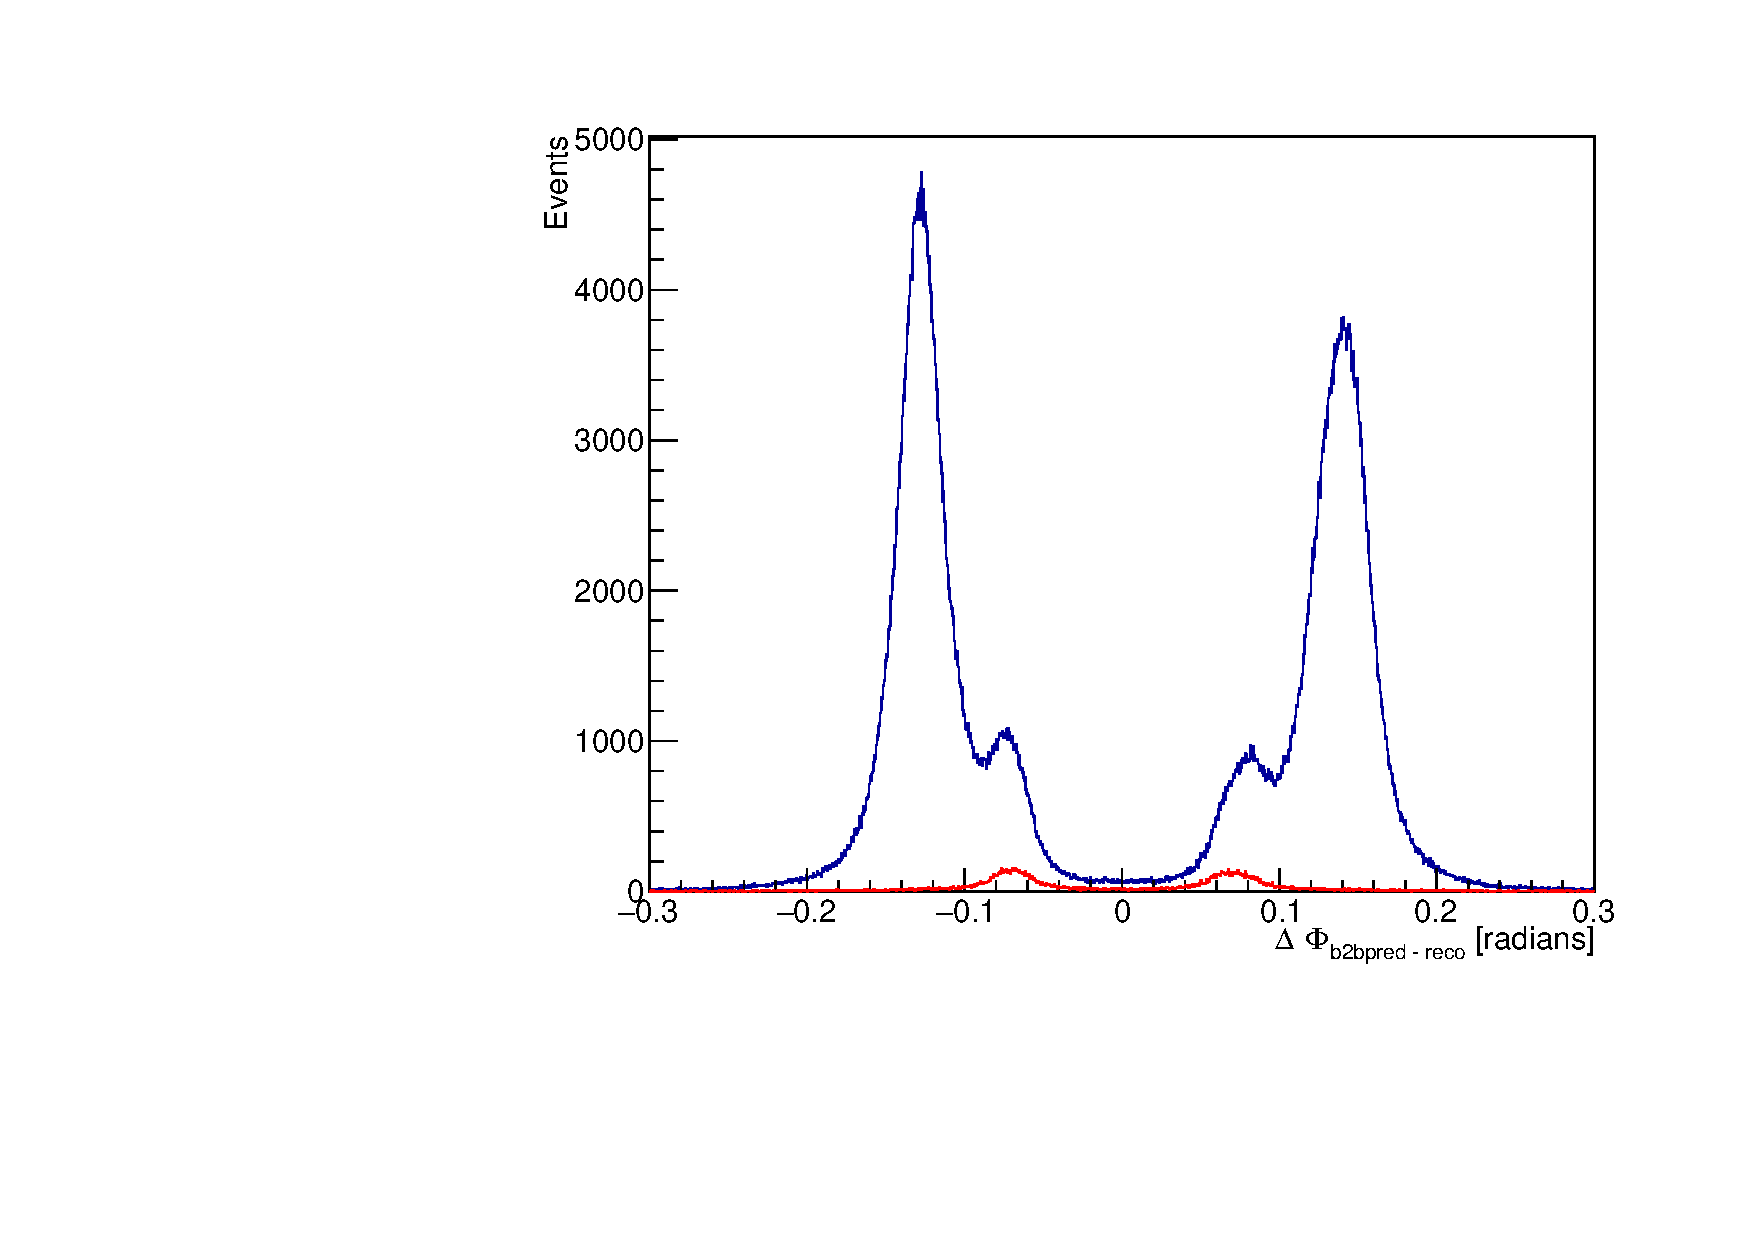
\includegraphics[width=4cm]{Plots/MCeg}
	\end{figure}
	
	\end{textblock*}	

\begin{textblock*}{\textwidth}(4cm,-0.5cm)
	\begin{figure}
		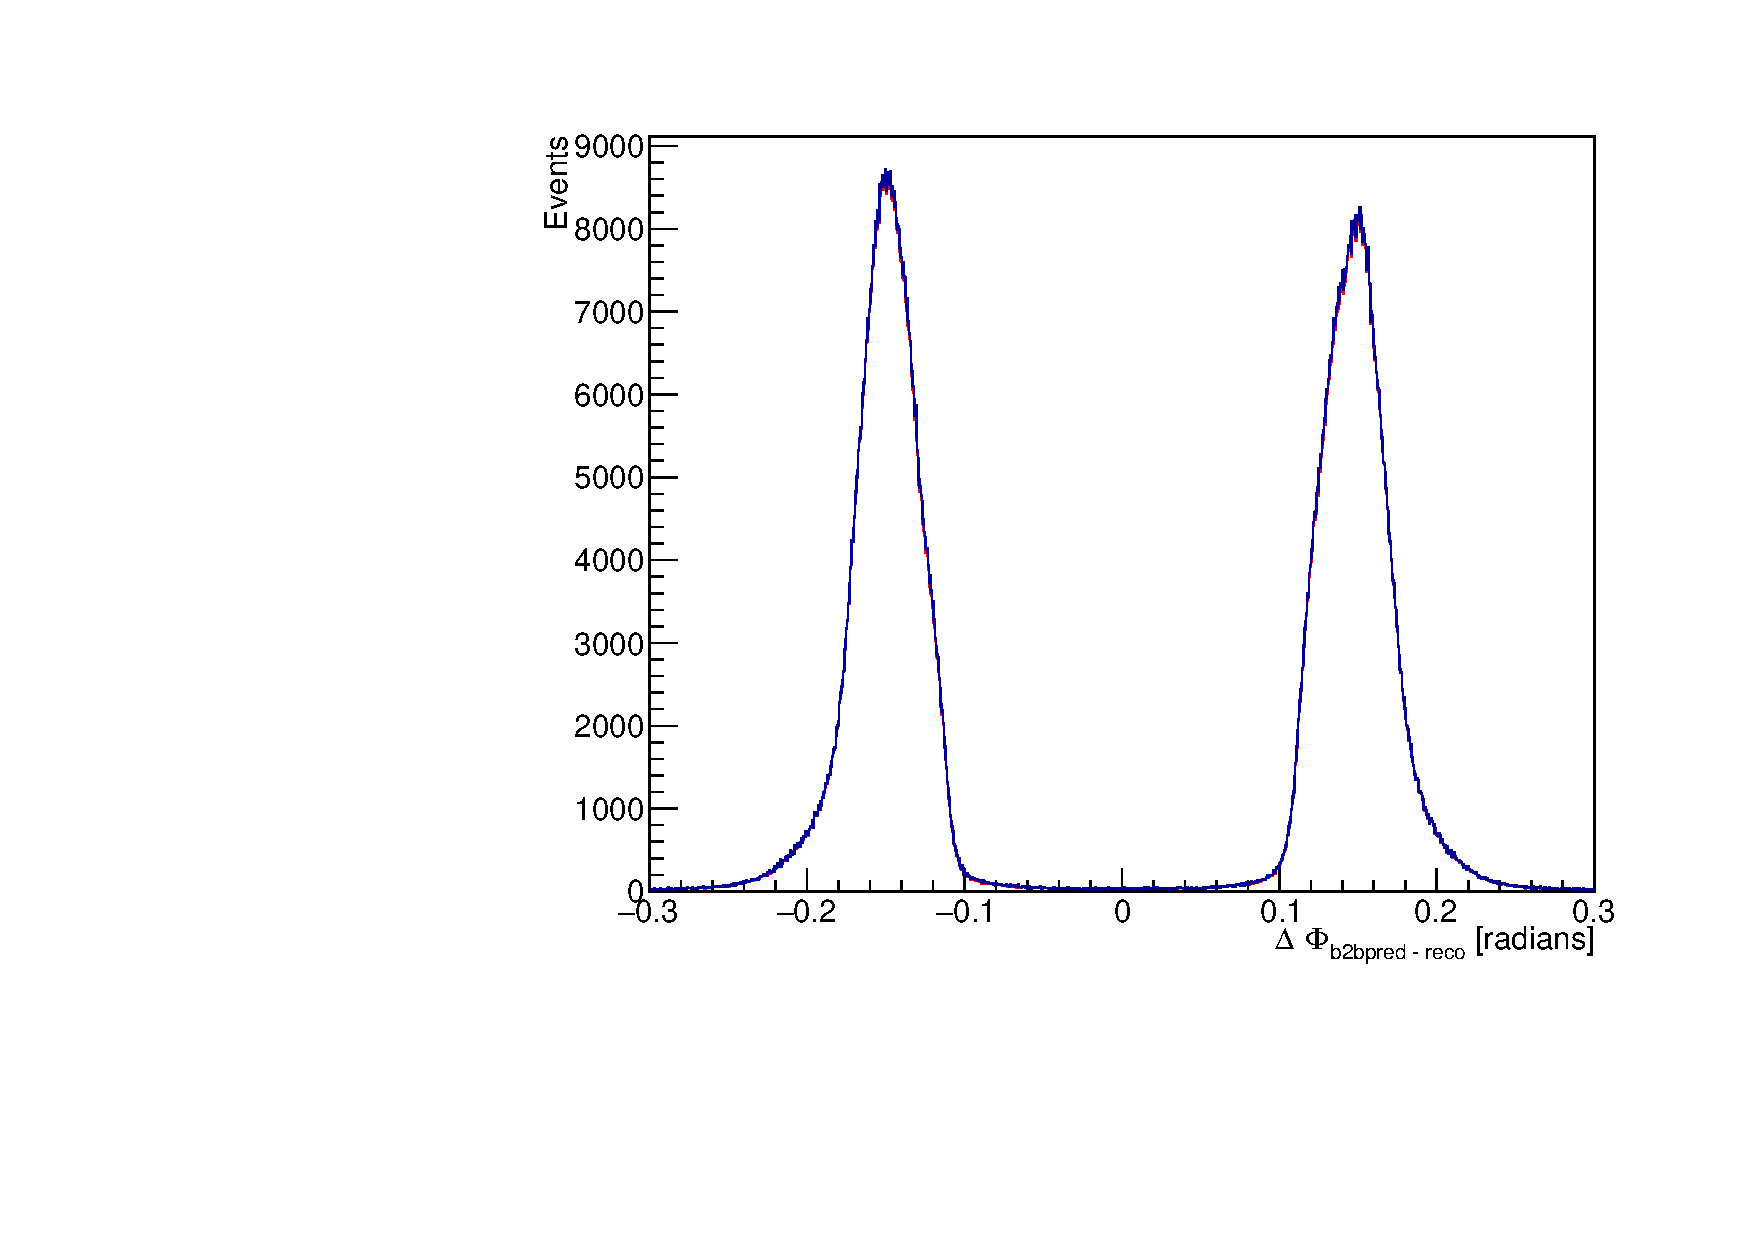
\includegraphics[width=4cm]{Plots/MCee}
	\end{figure}
	
\end{textblock*}	

\begin{textblock*}{\textwidth}(7.5cm,-3.35cm)
	\begin{itemize}
		\item MC11 $\textrm{ee} \rightarrow \textrm{ee}$ sample
		\item Reconstructed \textcolor{blue}{blue}
		\item MCTruthMatched \textcolor{red}{red}
	\end{itemize}
	
\end{textblock*}

\begin{textblock*}{\textwidth}(1.15cm,3.3cm)
 $\gamma \gamma$
\end{textblock*}

\begin{textblock*}{\textwidth}(5.2cm,3.3cm)
	$\gamma \textrm{e}$
\end{textblock*}

\begin{textblock*}{\textwidth}(9.25cm,3.3cm)
	$\textrm{ee}$
\end{textblock*}


\begin{textblock*}{\textwidth}(5.2cm,-3.6cm)
	all
\end{textblock*}


\end{frame}


\begin{frame}{Number of candidates}
	
	\begin{itemize}
		\item Number of reconstructed vpho per event is oftentimes bigger than 1
	\end{itemize}
	
	
	
		\begin{figure}
		\begin{subfigure}{.5\textwidth}
			\centering
			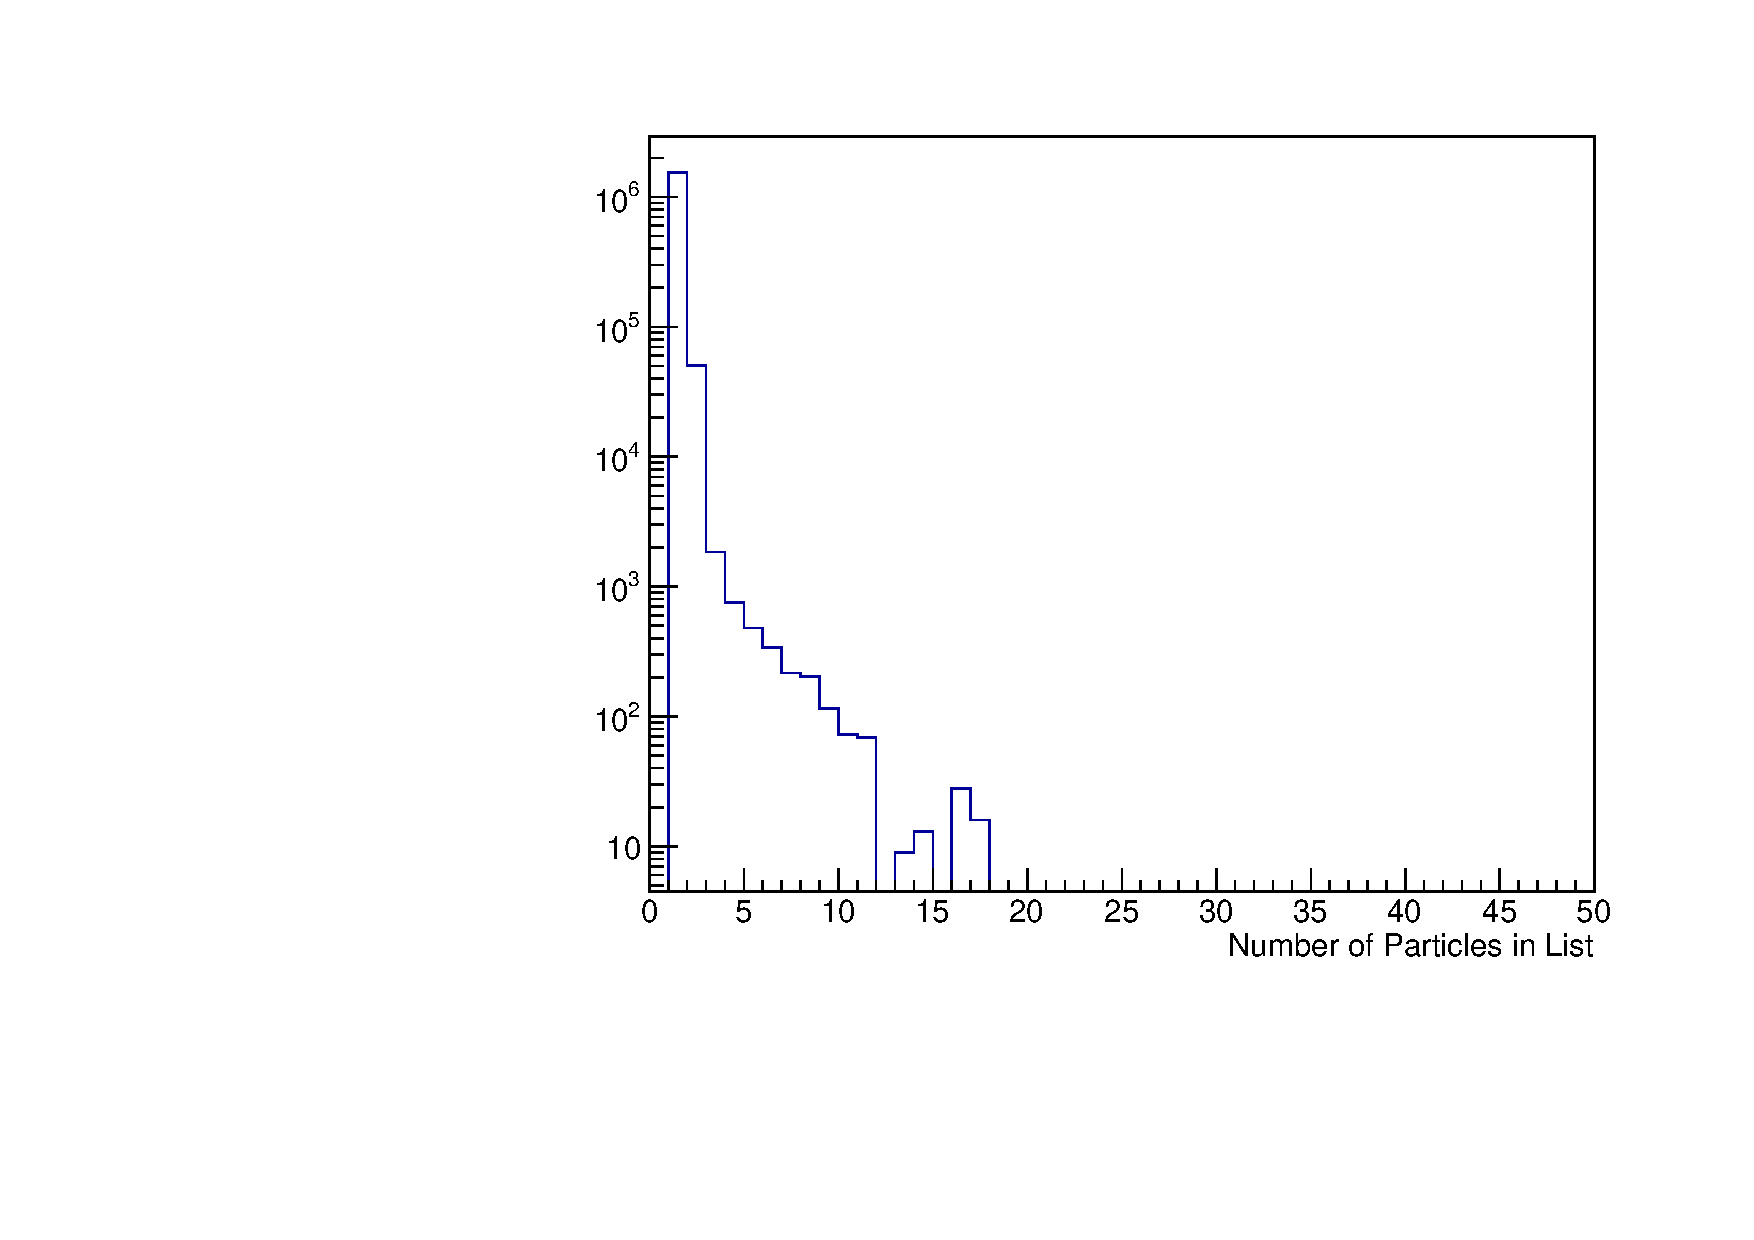
\includegraphics[width=4.5cm]{Plots/NumVpho}
			
			\label{fig:sub1}
		\end{subfigure}%
		\begin{subfigure}{.5\textwidth}
			\centering
			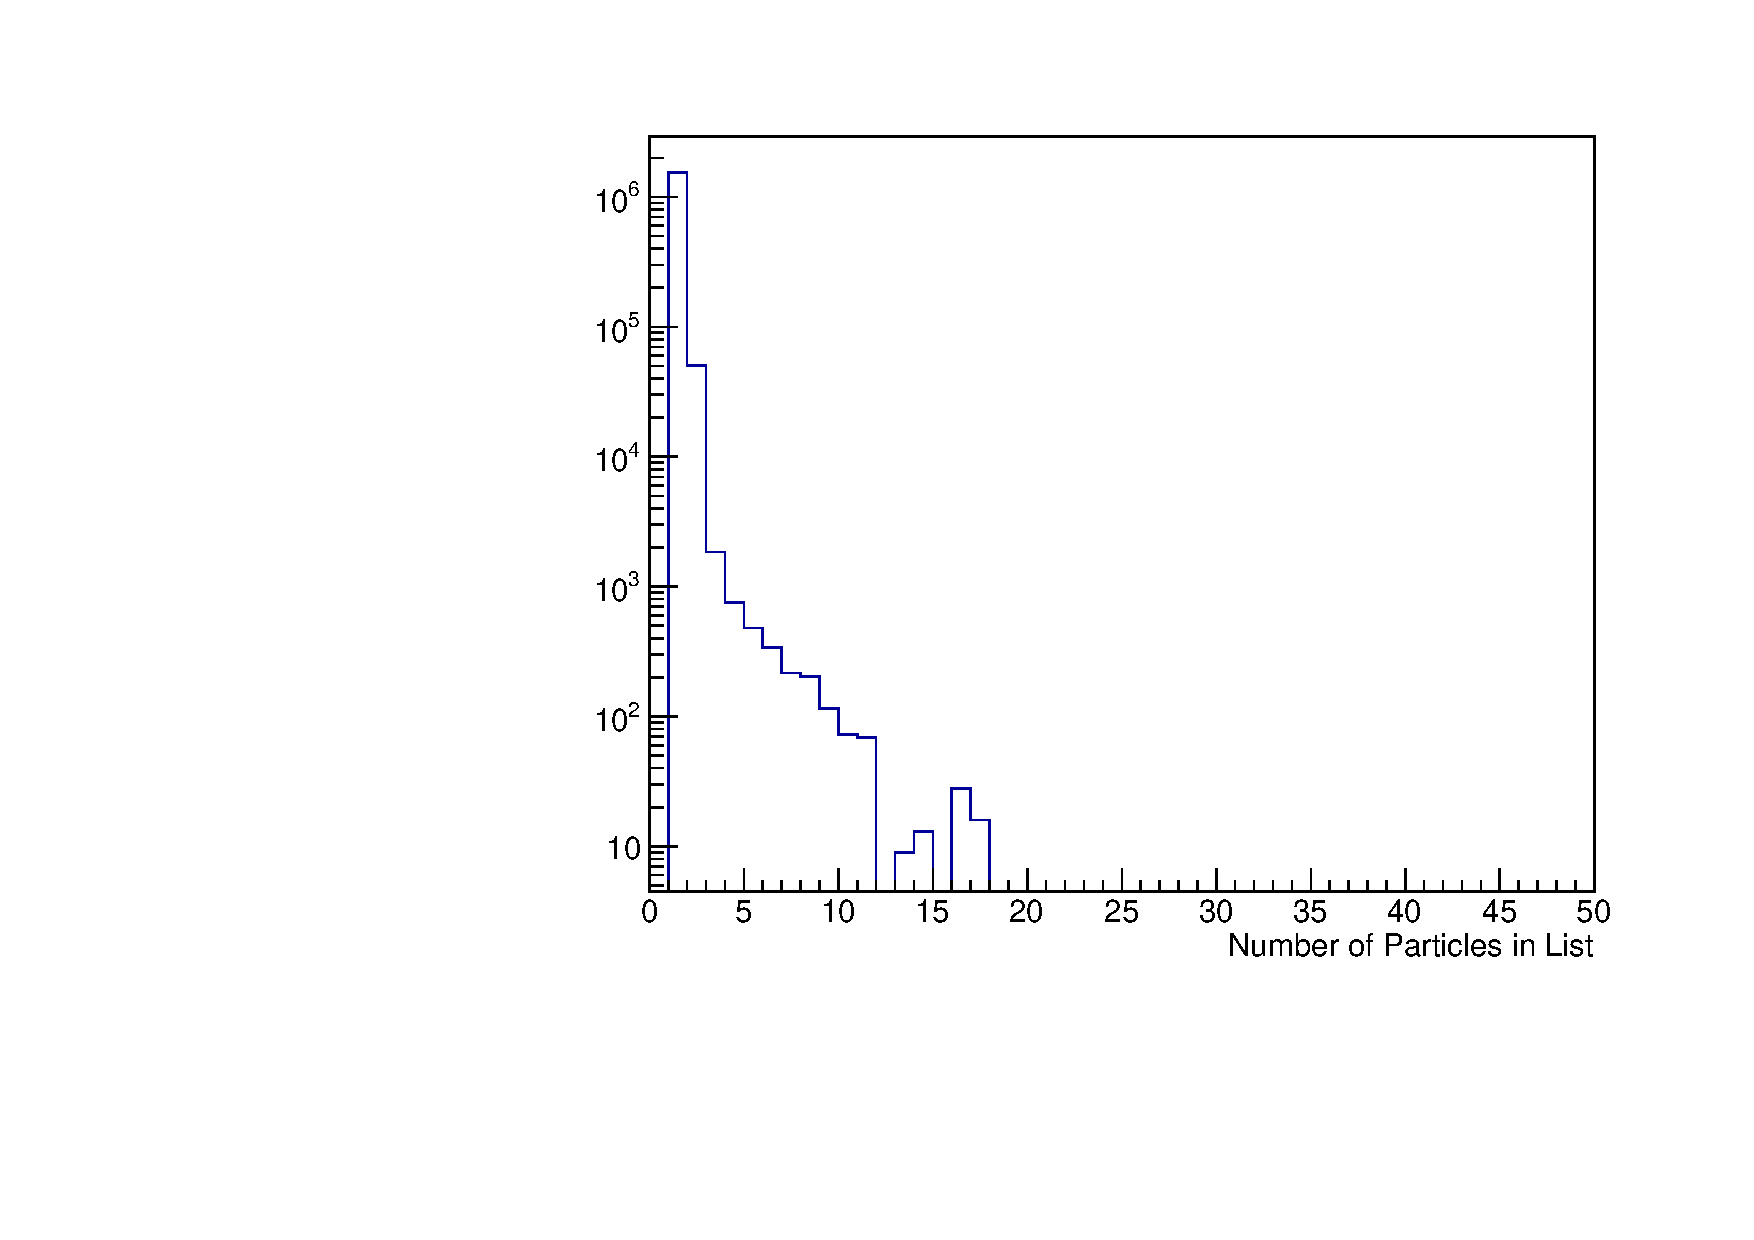
\includegraphics[width=4.5cm]{Plots/NumVphoMC}
			
			\label{fig:sub2}
		\end{subfigure}
		
		\label{fig:test}
	\end{figure}
	
	
\end{frame}



\begin{frame}{Next steps}
	\begin{itemize}
	\item Select best vpho
	\item Cut on $\Delta \Phi_{\textrm{b2bpred -reco}}$ peak and calculate a first efficiency
\end{itemize}
\end{frame}
\end{document}
